\documentclass[a4paper,11pt]{jlreq}

\usepackage{float}
\usepackage{graphicx}

\title{Taccovader game 説明書}
\date{\today}

\begin{document}
\maketitle

\section*{設定}
20xx年,地球は謎のタコ型宇宙人に攻め込まれそうになっていた...

そこで駆り出されたのがあなた! 宇宙船を操縦して迫りくる宇宙人を倒し,地球に平和をもたらしましょう!

\section*{登場するもの}
このゲームは画面上部から迫りくる敵を撃ち倒していくゲームです.
登場するオブジェクトは以下の通りです.
\begin{itemize}
\item プレイヤーが乗った宇宙船
\item 敵の攻撃を防ぐブロック
\item タコみたいな敵
\item 敵の弾
\item 宇宙船の波動弾
\end{itemize}

\begin{figure}[H]
    \centering
    \begin{minipage}{0.4\linewidth}
        \centering
        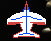
\includegraphics[width=\linewidth]{user.png}
        \caption{宇宙船}
        \label{fig:user}
    \end{minipage}
    \hfill
    \begin{minipage}{0.4\linewidth}
        \centering
        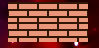
\includegraphics[width=\linewidth]{block.png}
        \caption{ブロック}
        \label{fig:block}
    \end{minipage}
\end{figure}

\subsection*{宇宙船}
プレイヤーが乗っている(ということになっている)宇宙船です. 敵との交戦中は左右には動けるので, 動きながら波動弾を発射して敵を倒しましょう!

\subsection*{ブロック}
敵の攻撃を防ぐことができるありがたいブロックです. この下に逃げ込んで敵の攻撃を避けましょう!


\begin{figure}[H]
    \centering
    \begin{minipage}{0.3\linewidth}
        \centering
        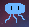
\includegraphics[width=\linewidth]{taccovader.png}
        \caption{敵}
        \label{fig:taccovader}
    \end{minipage}
    \hfill
    \begin{minipage}{0.3\linewidth}
        \centering
        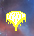
\includegraphics[width=\linewidth]{bullet.png}
        \caption{波動弾}
        \label{fig:bullet}
    \end{minipage}
    \hfill
    \begin{minipage}{0.3\linewidth}
        \centering
        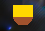
\includegraphics[width=\linewidth]{enemy_bullet.png}
        \caption{敵の弾}
        \label{fig:enemy_bullet}
    \end{minipage}
\end{figure}

\subsection*{敵}
青いタコみたいな敵. 波動弾で倒しましょう!

\subsection*{波動弾}
プレイヤーが乗っている宇宙船から発射される波動弾. 敵に当たると倒せます.

\subsubsection*{敵の弾}
銃弾みたいな弾を敵は発射してきます! うまく避けましょう!

\section*{遊び方}

5つステージが存在します. それらを順番にクリアしていきましょう!
ゲームの遊び方は以下のようになります.

まず, ダウンロードしたファイルを解凍した中に入っている図\ref{fig:application}のアプリをダブルクリックして実行します.
\begin{figure}[H]
    \centering
    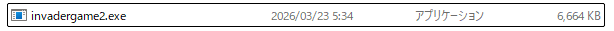
\includegraphics[width=\linewidth]{application.png}
    \caption{アプリケーション}
    \label{fig:application}
\end{figure}

そうすると図\ref{fig:title}のような画面になります. これがタイトル画面で, Sキーを押すとゲームプレイを開始できます.

\begin{figure}[H]
    \centering
    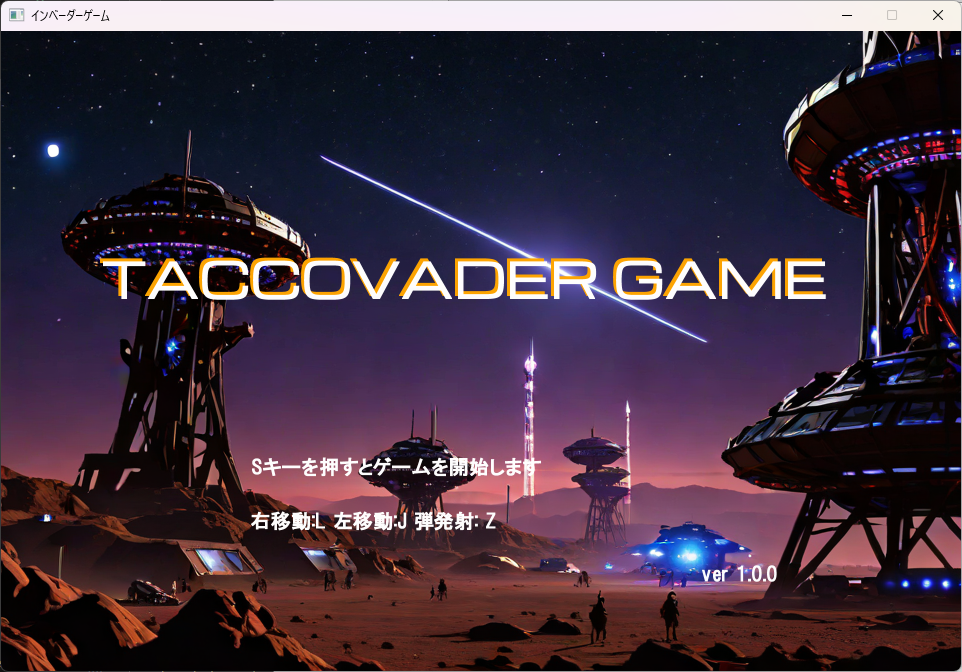
\includegraphics[width=0.7\linewidth]{title.png}
    \caption{タイトル画面}
    \label{fig:title}
\end{figure}

Sキーを押すと\ref{fig:play}のような1つ目のステージに遷移します. 左右に動きながら弾を発射して敵を倒しましょう!

\begin{figure}[H]
    \centering
    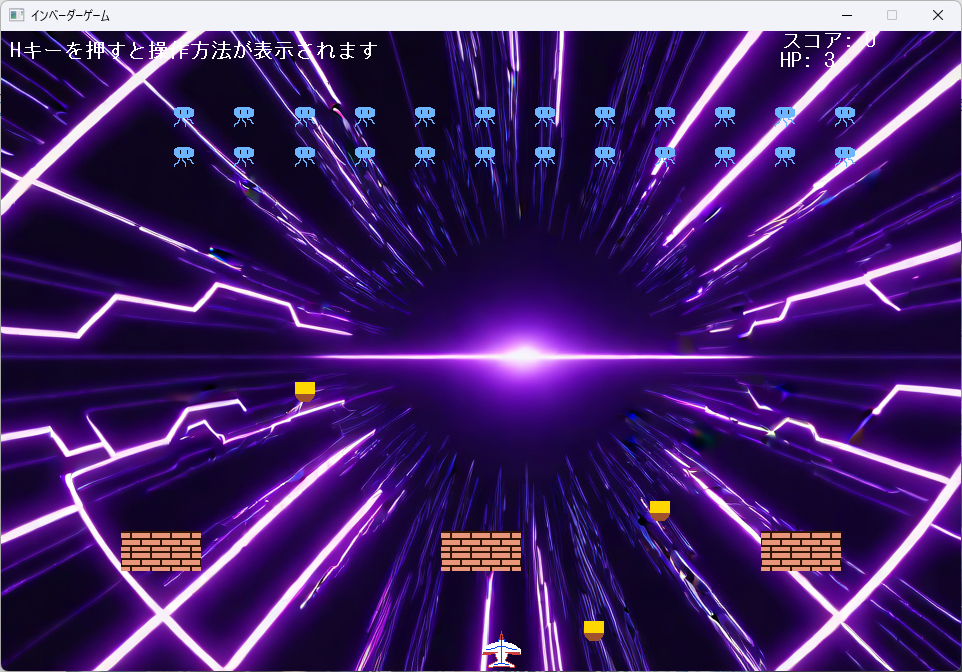
\includegraphics[width=0.7\linewidth]{play.png}
    \caption{ゲームプレイ中の画面}
    \label{fig:play}
\end{figure}

ステージをクリアした場合\ref{fig:clear}のような画面に移動します! Sキーを押せば次のステージに進むことができます!

\begin{figure}[H]
    \centering
    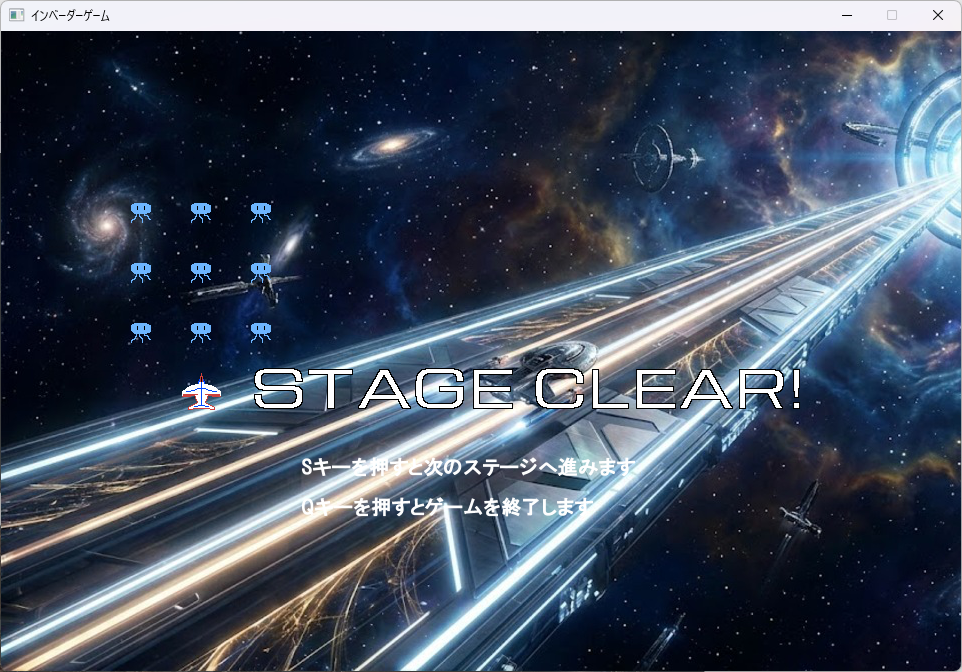
\includegraphics[width=0.7\linewidth]{clear.png}
    \caption{クリア画面}
    \label{fig:clear}
\end{figure}

惜しくも敵に敗れてしまった場合図\ref{fig:gameover}のような画面に遷移します. Sキーを押せば再度1つ目のステージから挑戦することができます!

\begin{figure}[H]
    \centering
    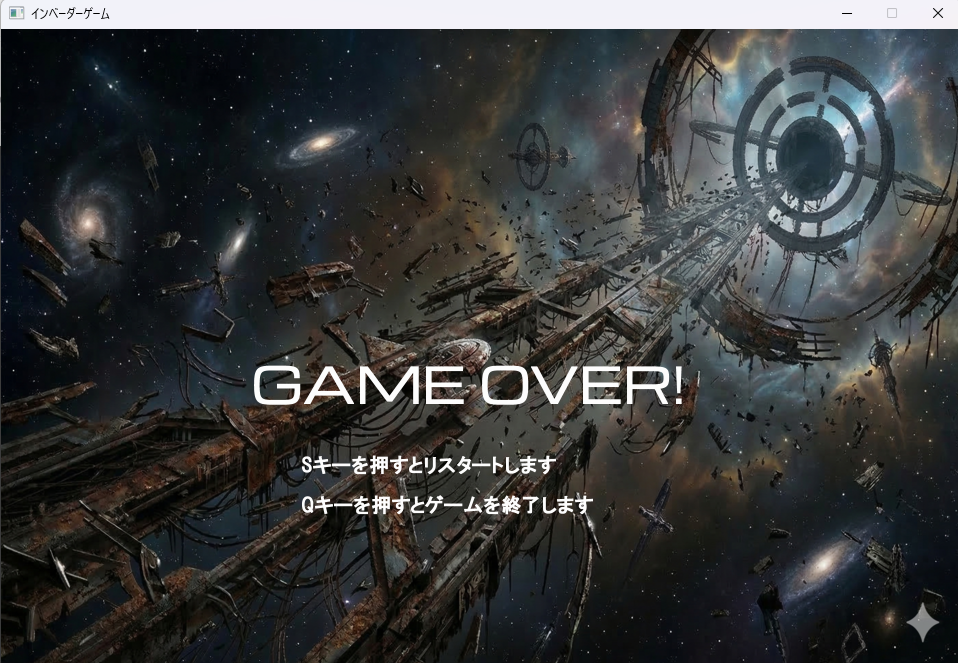
\includegraphics[width=0.7\linewidth]{gameover.png}
    \caption{ゲームオーバー画面}
    \label{fig:gameover}
\end{figure}

5つのステージ連続クリアを目指しましょう!


\section*{操作方法}
このゲームはキーボード操作のみでプレイすることができます. 操作方法は以下の通りです.

\begin{itemize}
    \item Lキー: 右移動
    \item Jキー: 左移動
    \item Zキー: 弾の射出
    \item Sキー, Qキー: 次のステージに進む/ゲームをやめる の選択
    \item Escキー: ゲームの終了
\end{itemize}







\end{document}


